\lab{K-Means Clustering}{K-Means Clustering}
\objective{Clustering is the one of the main tools in unsupervised learning---machine learning problems where the data comes without labels.
In this lab we implement the k-means algorithm, a simple and popular clustering method, and apply it to geographic clustering and color quantization.
}
\section*{Jupyter Notebooks}
Unlike previous labs where the python file submitted was a normal \li{.py} file, this lab among others will be done in a Jupyter Notebook (\li{.ipynb} or an iPython Notebook). 
Jupyter Notebooks is a powerful tool in visualizing data.
If you have used Google Colab, this works in a similar manner but it is run on your personal machine. 

Once Jupyter Notebook is installed, there are several ways of starting a Jupyter Notebook. 
The easiest way is to open a new terminal window and navigate to the directory with your .ipynb file, once in the desired directory, type Jupyter notebook.
This should automatically open a web browser to the Jupyter Notebook dashboard, from there you can select the .ipynb file and open and edit it.

The Python kernel will keep running in the background until told to stop.
So when you are done, to close the Jupyter Notebook, you need to go to file-> Close and Halt, or in the terminal window press ctrl+c (cmd+c for Mac). 

\begin{warn}
Before you push this file to Bitbucket to be graded, be sure to run each cell. 
When you push a .ipynb file, the current state of the file is pushed.
This means what you see is exactly what the graders will see.
\end{warn}


\section*{Clustering}

%Previously, we analyzed the iris dataset from \li{sklearn} using PCA; we have reproduced the first two principal components of the iris data in Figure \ref{fig:iris_data}.
%Upon inspection, a human can easily see that there are two very distinct groups of irises.
In this lab, we will analyze a few different datasets from Scikit-Learn's library and use the K-means algorithm. 
Figure \ref{fig:iris_data} is a graph of the iris dataset.
As a human, it is easy to identify the two distinct groups of data.
Can we create an algorithm to identify these groups without human supervision?
This task is called \emph{clustering}, an instance of \emph{unsupervised learning}.
The K-means algorithm is a simple way of helping computers see the group distinctions.

\begin{figure}
\centering
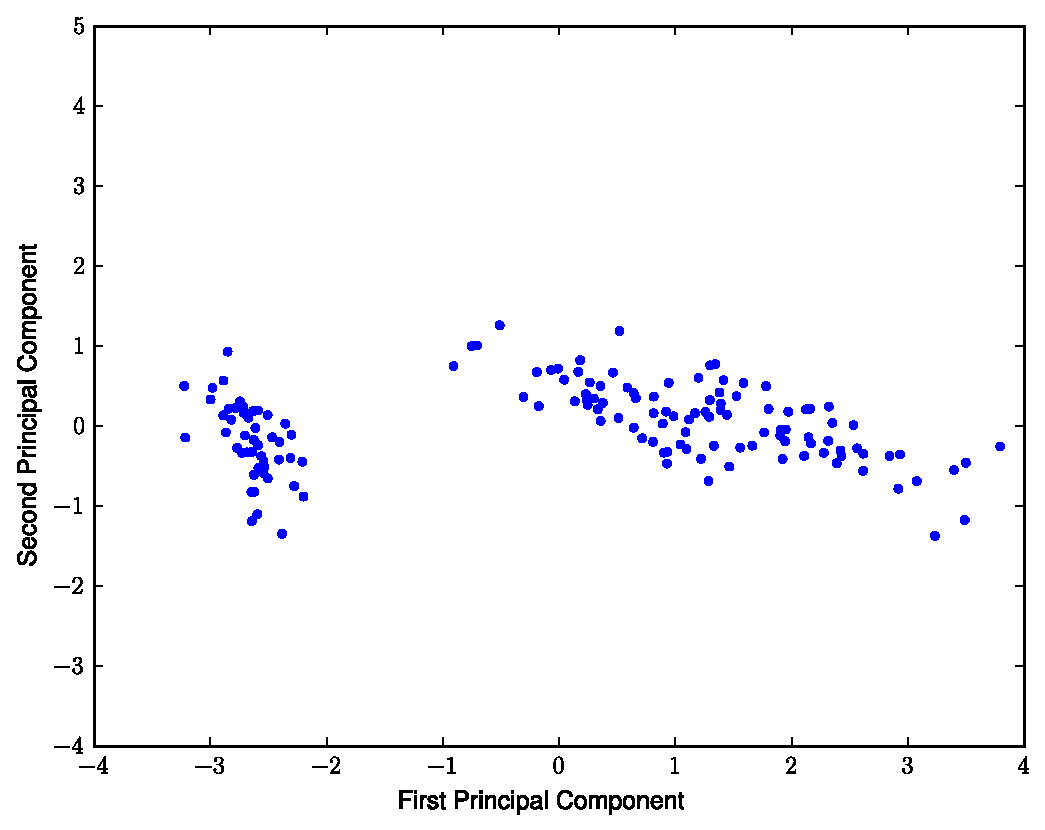
\includegraphics[width=.7\textwidth]{iris_pca.pdf}
\caption{The first two principal components of the iris dataset.}
\label{fig:iris_data}
\end{figure}

The objective of clustering is to find a partitions of the data such that points in the same subset will be ``close'' according to some metric.
The metric used will likely depend on the data, but some obvious choices include Euclidean distance and angular distance.
Throughout this lab, we will use the metric $d(x,y) = \|x-y\|_2$, the Euclidean distance between $x$ and $y$, unless we specify a different metric to be used.

More formally, suppose we have a collection of $\mathbb{R}^K$-valued observations $X = \{x_1,x_2,\ldots,x_n\}$.
Let $N \in \mathbb{N}$ and let $\mathcal{S}$ be the set of all $N$-partitions of $X$, where an $N$-partition is a partition with exactly $N$ nonempty elements.
We can represent a typical partition in $\mathcal{S}$ as $S = \{S_1,S_2,\ldots,S_N\}$, where
\[
X = \bigcup_{i=1}^N S_i
\]
and
\[
|S_i| > 0, \qquad i=1,2,\ldots,N.
\]
We seek the $N$-partition $S^*$ that minimizes the within-cluster sum of squares, i.e.
\[
S^* = \underset{S\in\mathcal{S}}{\arg\min} \sum_{i=1}^N\sum_{x_j\in S_i}\|x_j-\mu_i\|_2^2,
\]
where $\mu_i$ is the mean of the elements in $S_i$, i.e.
\[
\mu_i = \frac{1}{|S_i|}\sum_{x_j\in S_i}x_j.
\]

\subsection*{The K-Means Algorithm}

Finding the global minimizing partition $S^*$ is generally intractable since the set of partitions can be very large indeed,
but the \emph{k-means} algorithm is a heuristic approach that can often provide reasonably accurate results.


We begin by specifying an initial cluster mean $\mu_i^{(1)}$ for each $i = 1, \cdots, N$. 
This can be done by random initialization, or according to some heuristic.
For each iteration, we adopt the following procedure.
Given a current set of cluster means $\mu^{(t)}$, we find a partition $S^{(t)}$ of the observations such that
\begin{equation*}
S_{i}^{(t)} = \{x_j \; : \; \|x_j - \mu_{i}^{(t)}\|_2^2 \leq \|x_j - \mu_{l}^{(t)}\|_2^2,\,\,\,  l = 1, \cdots, N\}.
\end{equation*}
We then update our cluster means by computing for each $i = 1, \cdots, N$.
We continue to iterate in this manner until the partition ceases to change.


Figure \ref{fig:iris_clusterings} shows two different clusterings of the iris data produced by the \emph{k-means} algorithm.
Note that the quality of the clustering can depend heavily on the initial cluster means.
We can use the within-cluster sum of squares as a measure of the quality of a clustering (a lower sum of squares is better).
Where possible, it is advisable to run the clustering algorithm several times, each with a different initialization of the means,
and keep the best clustering.
Note also that it is possible to have very slow convergence.
Thus, when implementing the algorithm, it is a good idea to terminate after some specified maximum number of iterations.
%
\begin{figure}[h]
    \centering
    \begin{tabular}{cc}
    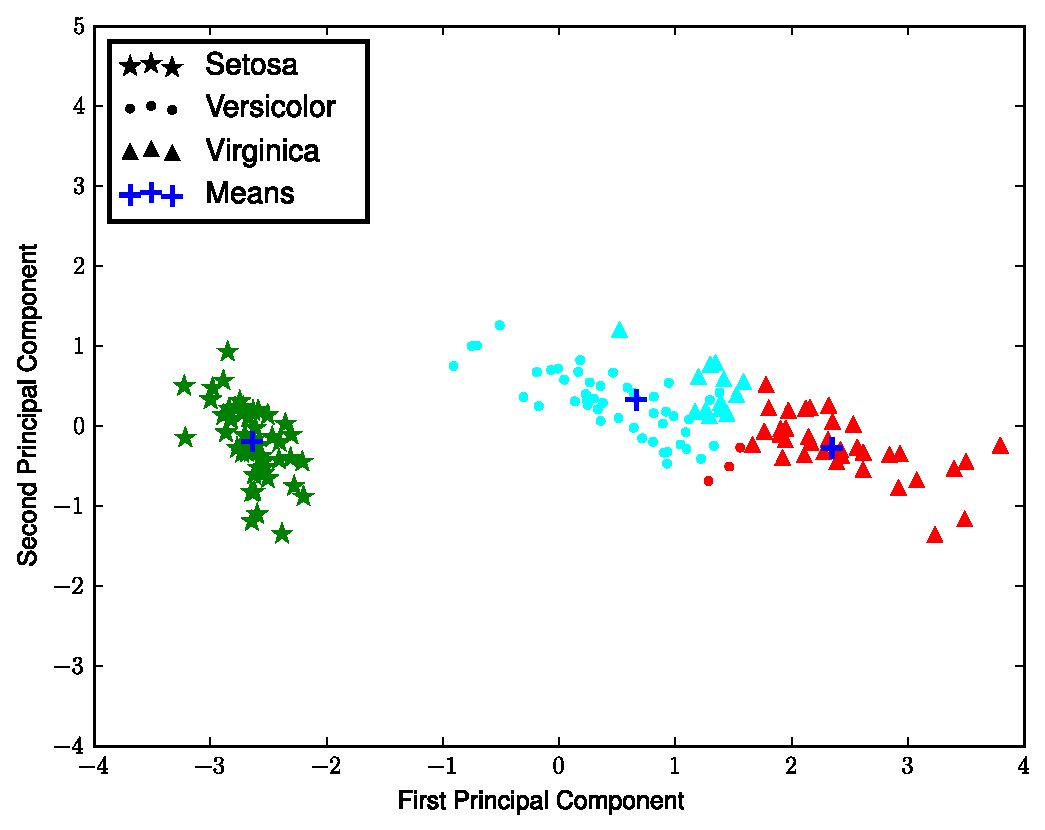
\includegraphics[width=.49\textwidth]{iris_means_1.pdf} &
    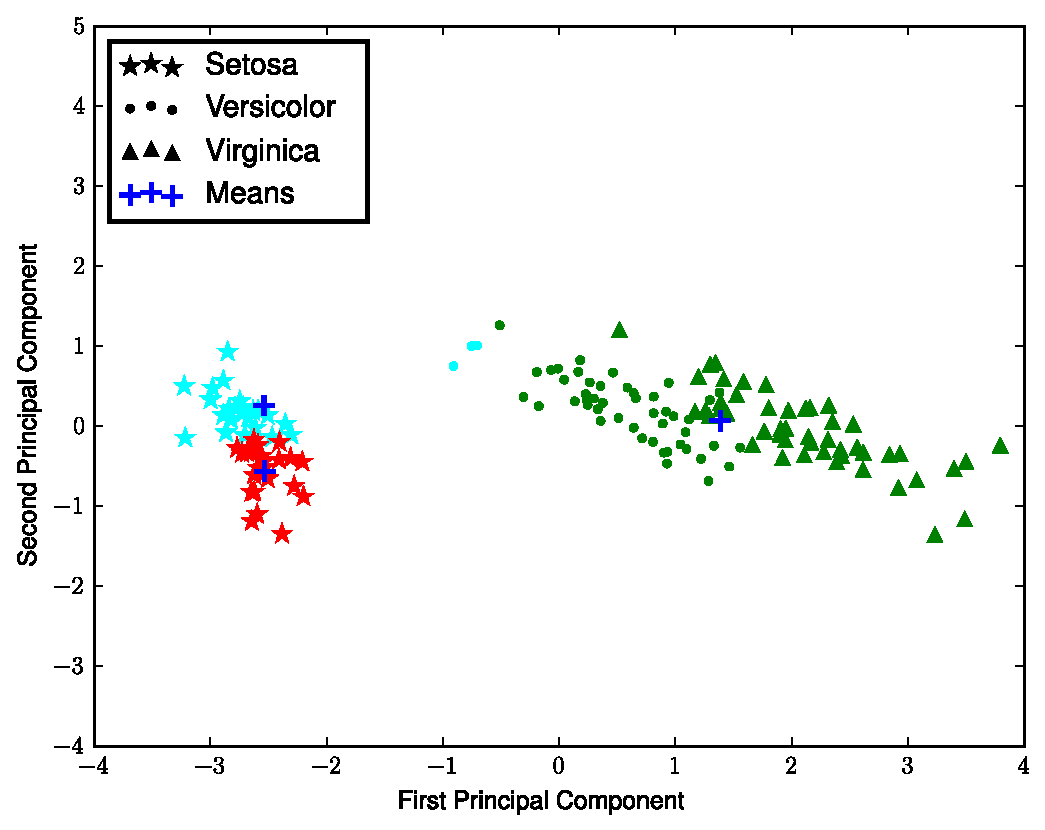
\includegraphics[width=.49\textwidth]{iris_means_2.pdf}
    \end{tabular}
    \caption{Two different K-Means clusterings for the iris dataset.
            Notice that the clustering on the left predicts the flower species to a high degree of accuracy,
            while the clustering on the right is less effective.}
    \label{fig:iris_clusterings}
\end{figure}

The algorithm can be summarized as follows.
\begin{enumerate}
    \item From the data points, choose $k$ initial cluster centers.
    \item For $i=0,\ \ldots,$\ \li{max_iter},
    \begin{enumerate}
        \item Assign each data point to the cluster center that is closest, forming $k$ clusters.
        \item Recompute the cluster centers as the means of the new clusters.
        \item If the old cluster centers and the new cluster centers are sufficiently close, terminate early.
    \end{enumerate}
\end{enumerate}


%\Procedure{K-Means Algorithm}{$X$}
%    \State Random\_ints $\gets$ n\_cluster random integers
%    \State Centers = 
%    \State $n \gets \text{length}(X)$
%    \For{$k = 0,\ 1,\ \ldots,\ max\_iter$}
%    	 \State \text{Calculate distances from each point to each center}
%    	 
%    \EndFor
%   
%    \State Do steps \ref{}--\ref{} of Algorithm \ref{} to get the eigenvalues of $S$.
%\subsection*{The Algorithm}
%\begin{itemize}
%\item Choose n random data points to be your initial centers.
%\item Calculate the distance from each point to each center.
%\item Put the data into the groups with the same closest centers.
%\item For each group, find the centroid and use these new points as new your new centers.
%\item Repeat this process until the centers have come to an equilibrium given some tolerance or the max iterations is reached. 
%\end{itemize}

\begin{problem}
Write a \li{KMeans} class for doing basic $k$-means clustering.
Implement the following methods, following \li{sklearn} class conventions.
\begin{enumerate}
\item \li{__init__()}: Accept a number of clusters $k$, a maximum number of iterations, and a convergence tolerance.
Store these as attributes.

\item \li{fit()}: Accept an $m \times n$ matrix $X$ of $m$ data points with $n$ features.
Choose $k$ random rows of $X$ as the initial cluster centers.
Run the $k$-means iteration until consecutive centers are within the convergence tolerance, or until iterating the maximum number of times.
Save the cluster centers as attributes.

If a cluster is empty, reassign the cluster center as a random row of $X$.

\item \li{predict()}: Accept an $l \times n$ matrix $X$ of data.
Return an array of $l$ integers where the $i$th entry indicates which cluster center the $i$th row of $X$ is closest to.
\end{enumerate}
%
Test your class on the iris data set after reducing the data to two principal components.
Plot the data, coloring by cluster.
\end{problem}

\section*{Fire Station Placement} %=============================================
When urban planners are making plans for a city, there are many city elements to consider. 
One of which is the locations of the fire stations that will service the city.
When choosing a suitable location for the city, urban planners look at the current building locations, the roads nearby each location, prior traffic history and the areas of potential growth.
We will simplify this complex problem by only taking into account the distances from each building to the nearest fire station (see Additional Material for a harder version of this problem).

Using another data set from SKLearn, we can get the data from the 1990 US Census for California housing based on the blocks of the residents.
This has been saved in \texttt{sacramento.npy} and can be accessed by using the np.load() function.
This file contains demographic data for each block in Sacramento and nearby cities. 
The eight columns in the file are: median block income, median house age in the block, average number of rooms, average number of bedrooms, average house occupancy, latitude and longitude.

There are couple ways for a fire station to be optimally placed. 
The stations could be placed to minimize the average distance to each house.
Another option is to minimize the distance to the farthest house in each group.
For this problem, minimize the distance to the farthest house in each group.

\begin{problem}
Using the Methods you wrote in Problem 1, add a parameter, p, to your class that denotes the norm and defaults to 2.
Save p as an attribute to be used in your fit() and predict() functions.
Using the data in \texttt{sacramento.npy} find the optimal placement for the fire stations. 
Plot the longitude and latitudes, the centers, and color them by cluster.
Try different values for \texttt{p} to find the optimal locations for the fire stations.
As the initial centers are chosen at random, make sure to run the \texttt{predict()} function several times.
In a Markdown cell report which norm was the best at keeping the maximum distance small.

\end{problem}
\begin{figure}[H]
	\centering
	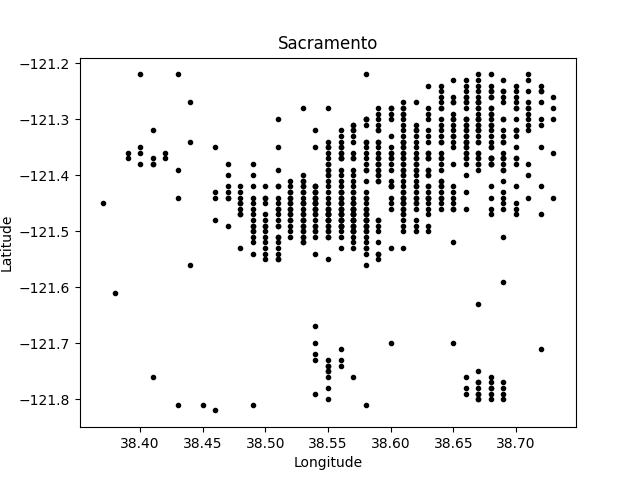
\includegraphics[width=.7\textwidth]{sacramento.png}
	\caption{Sacramento Housing Data (1990 US Census).}
	\label{fig:sacramento}
\end{figure}

\section*{Detecting Active Earthquake Regions} % ==============================

Suppose we are interested in learning about which regions are prone to experience frequent earthquake activity.
We could make a map of all earthquakes over a given period of time and examine it ourselves, but this, as an unsupervised learning problem, can be solved using our $k$-means clustering tool.

% % Old approach (required students to parse 6 files for some reason).
% These files contain a lot of information which isn't of interest to us at the present time; all we would like to extract from them is the location of each earthquake, which appears in characters $21$ through $33$ of each line.
% Characters $21$ through $26$ contain the latitude of each epicenter, character $26$ denoting North or South, and characters $27$ through $33$ contain the longitude of each epicenter, character $33$ denoting East or West.
% We need to divide each value by $1,000$ to represent these as degrees and decimals.
\begin{figure}[H]
    \centering
    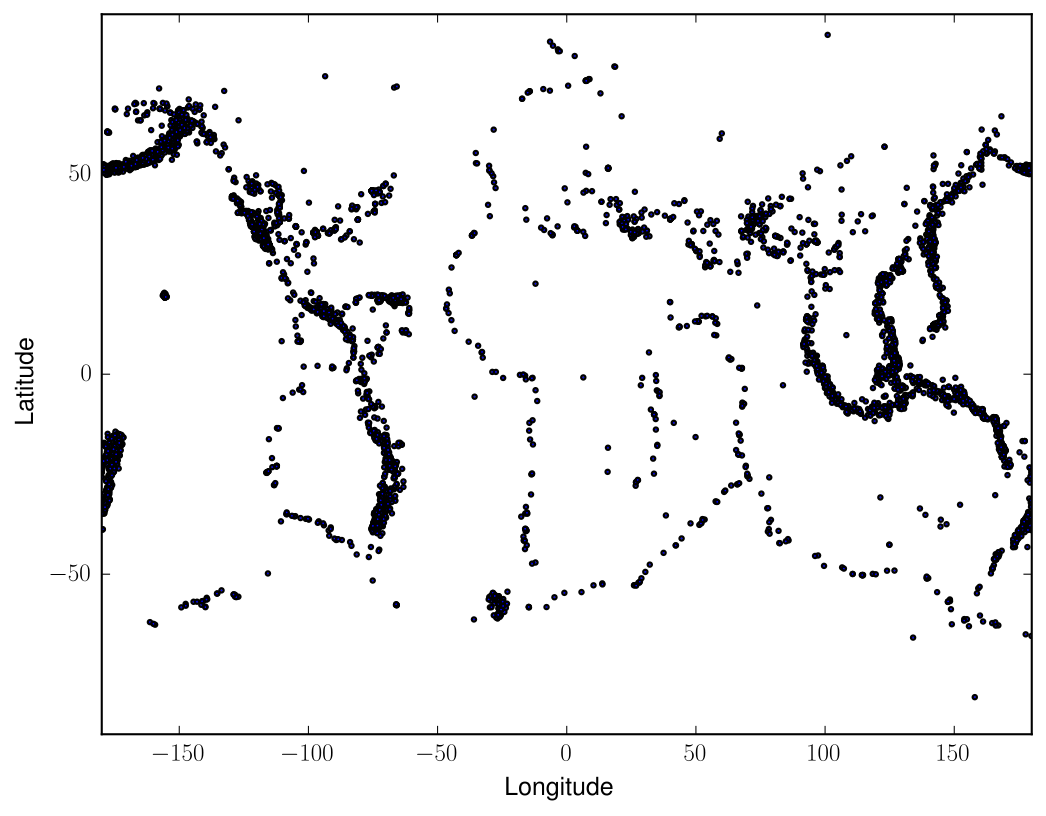
\includegraphics[width=.7\textwidth]{earthquakes.png}
    \caption{Earthquake epicenters over a 6 month period.}
    \label{fig:earthquakes}
\end{figure}

The file \texttt{earthquake\_coordinates.npy} contains earthquake data throughout the world from January 2010 through June 2010.
Each row represents a different earthquake; the columns are scaled longitude and latitude measurements.
We want to cluster this data into active earthquake regions.
For this task, we might think that we can regard any epicenter as a point in $\mathbb{R}^{2}$ with coordinates being their latitude and longitude.
This, however, would be incorrect, because the earth is not flat.
Instead, latitude and longitude should be viewed in \emph{spherical coordinates} in $\mathbb{R}^{3}$, which could then be clustered.

A simple way to accomplish this transformation is to first transform the latitude and longitude values to spherical coordinates, and then to Euclidean coordinates.
Recall that a spherical coordinate in $\mathbb{R}^3$ is a triple $(r,\theta,\varphi)$, where $r$ is the distance from the origin, $\theta$ is the radial angle in the $xy$-plane from the $x$-axis, and $\varphi$ is the angle from the $z$-axis.
In our earthquake data, once the longitude is converted to radians it is an appropriate $\theta$ value; the latitude needs to be offset by $90^\circ$ degrees, then converted to radians to obtain $\varphi$.
For simplicity, we can take $r=1$, since the earth is roughly a sphere.
We can then transform to Euclidean coordinates using the following relationships.
\[
\theta = \frac{\pi}{180}\left(\text{longitude}\right)
\qquad
\varphi = \frac{\pi}{180}\left(90 - \text{latitude}\right)
\]
\begin{align*}
r & = \sqrt{x^{2} + y^{2} + z^{2}} & x & = r \sin \varphi \cos \theta \\
\varphi & = \arccos \frac{z}{r} & y & = r \sin \varphi \sin \theta \\
\theta & = \arctan \frac{y}{x} & z & = r \cos \varphi
\end{align*}

There is one last issue to solve before clustering.
Each earthquake data point has norm 1 in Euclidean coordinates, since it lies on the surface of a sphere of radius 1.
Therefore, the cluster centers should also have norm 1.
Otherwise, the means can't be interpreted as locations on the surface of the earth, and the \emph{k-means} algorithm will struggle to find good clusters.
A solution to this problem is to normalize the mean vectors at each iteration, so that they are always unit vectors.

\begin{problem}
Add a keyword argument \li{normalize=False} to your \li{KMeans} constructor.
Modify \li{fit()} so that if \li{normalize} is \li{True}, the cluster centers are normalized at each iteration.

Cluster the earthquake data in three dimensions by converting the data from raw data to spherical coordinates to euclidean coordinates on the sphere.
\begin{enumerate}
\item Convert longitude and latitude to radians, then to spherical coordinates.
\\(Hint: \li{np.deg2rad()} may be helpful.)
\item Convert the spherical coordinates to euclidean coordinates in $\mathbb{R}^3$.
\item Use your \li{KMeans} class with normalization to cluster the euclidean coordinates.
\item Translate the cluster center coordinates back to spherical coordinates, then to degrees.
Transform the cluster means back to latitude and longitude coordinates.
\\(Hint: use \li{numpy.arctan2()} for $\arctan$, so that that correct quadrant is chosen).
\item Plot the data, coloring by cluster.
Also mark the cluster centers.
\end{enumerate}
With 15 clusters, your plot should resemble the Figure \ref{fig:earthquakeclusters}.
\end{problem}

\begin{figure}[H]
    \centering
    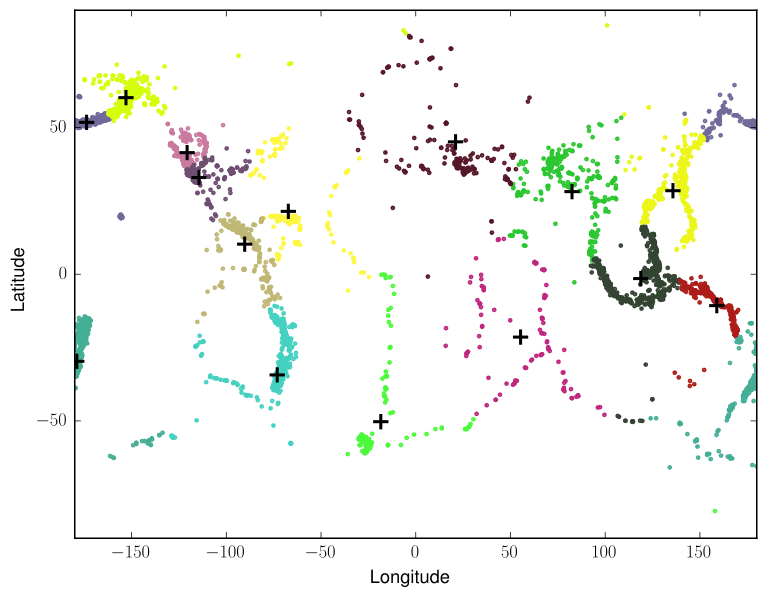
\includegraphics[width=.7\textwidth]{earthquake_clusters.png}
    \caption{Earthquake epicenter clusters with $k = 15$.}
    \label{fig:earthquakeclusters}
\end{figure}

\begin{comment}
Though plotting our results in two dimensions gives us a good picture, we can see that this is not entirely accurate.  There are points that appear to be closer to a different cluster center than the one to which they belong.  This comes from viewing the results in only two dimensions.  When viewing in three dimensions, we can see more clearly the accuracy of our results.
\begin{problem}
Add a keyword argument \li{3d=False} to your \li{kmeans} function, and add code to show the three-dimensional plot instead of the two-dimensional scatter plot should this argument be set to \li{True}.  Maintain the same color-coding scheme as before.
\end{problem}
\end{comment}




\section*{Color Quantization} % ===============================================

The $k$-means algorithm uses the euclidean metric, so it is natural to cluster geographic data.
However, clustering can be done in any abstract vector space.
The following application is one example.

Images are usually represented on computers as $3$-dimensional arrays.
Each $2$-dimensional layer represents the red, green, and blue color values, so each pixel on the image is really a vector in $\mathbb{R}^3$.
Clustering the pixels in $RGB$ space leads a one kind of image segmentation that facilitate memory reduction.

Reading: \url{https://en.wikipedia.org/wiki/Color_quantization}

\begin{problem}
Write a function that accepts an image array (of shape $(m,n,3)$), an integer number of clusters $k$, and an integer number of samples $S$.
Reshape the image so that each row represents a single pixel.
Choose $S$ pixels to train a $k$-means model on with $k$ clusters.
Make a copy of the original picture where each pixel has the same color as its cluster center.
Return the new image.
For this problem, you may use \li{sklearn.cluster.KMeans} instead of your \li{KMeans} class from Problem 1.

Test your function on some of the provided NASA images.
\end{problem}

\newpage

\section*{Additional Material} % ==============================================

\subsection*{Spectral Clustering}
We now turn to another method for solving a clustering problem, namely that of Spectral Clustering.  As you can see in Figure ???, it can cluster data not just by its location on a graph, but can even separate shapes that overlap others into distinct clusters.  It does so by utilizing the spectral properties of a Laplacian matrix.  Different types of Laplacian matrices can be used.  In order to construct a Laplacian matrix, we first need to create a graph of vertices and edges from our data points.  This graph can be represented as a symmetric matrix $W$ where $w_{ij}$ represents the edge from $x_i$ to $x_j$.  In the simplest approach, we can set $w_{ij} = 1$ if there exists an edge and $w_{ij} = 0$ otherwise.  However, we are interested in the similarity of points, so we will weight the edges by using a \emph{similarity measure}.  Points that are similar to one another are assigned a high similarity measure value, and dissimilar points a low value.  One possible measure is the \emph{Gaussian similarity function}, which defines the similarity between distinct points $x_i$ and $x_j$ as
\begin{equation*}
s(x_i,x_j) = e^{- \frac{\| x_i - x_j \| ^2}{2 \sigma ^2}}
\end{equation*}
for some set value $\sigma$.

Note that some similarity functions can yield extremely small values for dissimilar points.  We have several options for dealing with this possibility.  One is simply to set all values which are less than some $\epsilon$ to be zero, entirely erasing the edge between these two points.  Another option is to keep only the $T$ largest-valued edges for each vertex.  Whichever method we choose to use, we will end up with a weighted \emph{similarity matrix} $W$.  Using this we can find the diagonal \emph{degree matrix} $D$, which gives the number of edges found at each vertex.  If we have the original fully-connected graph, then $D_{ii} = n-1$ for each $i$.  If we keep the $T$ highest-valued edges, $D_{ii} = T$ for each $i$.

As mentioned before, we may use different types of Laplacian matrices.  Three such possibilities are:
\begin{enumerate}
    \item The \emph{unnormalized Laplacian}, $L = D - W$
    \item The \emph{symmetric normalized Laplacian}, $L_{sym} = I - D^{-1/2}WD^{-1/2}$
    \item The \emph{random walk normalized Laplacian}, $L_{rw} = I - D^{-1}W$.
 \end{enumerate}

Given a similarity measure, which type of Laplacian to use, and the desired number of clusters $k$, we can now proceed with the Spectral Clustering algorithm as follows:

\begin{itemize}
    \item Compute $W$, $D$, and the appropriate Laplacian matrix.
    \item Compute the first $k$ eigenvectors $u_1, \cdots , u_k$ of the Laplacian matrix.
    \item Set $U = [u_1, \cdots , u_k]$, and if using $L_{sym}$ or $L_{rw}$ normalize $U$ so that each row is a unit vector in the Euclidean norm.
    \item Perform $k$-means clustering on the $n$ rows of $U$.
    \item The $n$ labels returned from your \li{kmeans} function correspond to the label assignments for $x_1, \cdots, x_n$.
\end{itemize}

As before, we need to run through our $k$-means function multiple times to find the best measure when we use random initialization.  Also, if you normalize the rows of $U$, then you will need to set the argument \li{normalize = True}.

\begin{problem}
Implement the Spectral Clustering Algorithm by calling your \li{kmeans} function, using the following function declaration:
\begin{lstlisting}
def specClus(measure,Laplacian,args,arg1=None,kiters=10):
    """
    Cluster a dataset using the k-means algorithm.

    Parameters
    ----------
    measure : function
        The function used to calculate the similarity measure.
    Laplacian : int in {1,2,3}
        Which Laplacian matrix to use. 1 corresponds to the unnormalized,
        2 to the symmetric normalized, 3 to the random walk normalized.
    args : tuple
        The arguments as they were passed into your k-means function,
        consisting of (data, n_clusters, init, max_iter, normalize). Note
        that you will not pass 'data' into your k-means function.
    arg1 : None, float, or int
        If Laplacian==1, it should remain as None
        If Laplacian==2, the cut-off value, epsilon.
        If Laplacian==3, the number of edges to retain, T.
    kiters : int
        How many times to call your kmeans function to get the best
        measure.

    Returns
    -------
    labels : ndarray of shape (n,)
        The i-th entry is an integer in [0,n_clusters-1] indicating
        which cluster the i-th row of data belongs to.
    """
    pass
\end{lstlisting}
\end{problem}

We now need a way to test our code.  The website http://cs.joensuu.fi/sipu/datasets/ contains many free data sets that will be of use to us.  Scroll down to the ``Shape sets" heading, and download some of the datasets found there to use for trial datasets.
\begin{problem}
Create a function that will return the accuracy of your spectral clustering implementation, as follows:
\begin{lstlisting}
def test_specClus(location,measure,Laplacian,args,arg1=None,kiters=10):
    """
    Cluster a dataset using the k-means algorithm.

    Parameters
    ----------
    location : string
        The location of the dataset to be tested.
    measure : function
        The function used to calculate the similarity measure.
    Laplacian : int in {1,2,3}
        Which Laplacian matrix to use. 1 corresponds to the unnormalized,
        2 to the symmetric normalized, 3 to the random walk normalized.
    args : tuple
        The arguments as they were passed into your k-means function,
        consisting of (data, n_clusters, init, max_iter, normalize). Note
        that you will not pass 'data' into your k-means function.
    arg1 : None, float, or int
        If Laplacian==1, it should remain as None
        If Laplacian==2, the cut-off value, epsilon.
        If Laplacian==3, the number of edges to retain, T.
    kiters : int
        How many times to call your kmeans function to get the best
        measure.

    Returns
    -------
    accuracy : float
        The percent of labels correctly predicted by your spectral
        clustering function with the given arguments (the number
        correctly predicted divided by the total number of points.
    """
    pass
\end{lstlisting}
\end{problem}

\subsection*{Fire Station Placement II}
In problem 2 we looked at choosing the best location for a fire station. 
However, because we looked at the city of Sacramento where the geography doesn't role in choosing a location, we didn't need to double check that there is a place for the station.
The \li{sanfrancisco.npy} data is organized the same way as \li{sacramento.py}, as this also comes from the SKLearn California Housing Module.
Doing the same method as before will give us groups of houses, however, the group centers may be in the middle of the bay.
When implementing this problem, perform a check on the centers to make sure they are not in water. 
The file \li{bayboundary.npy} gives a rough outline of where the bay is.
The \li{bayboundary.npy} has only 2 columns, longitude and latitude.
Using the boundaries set, make sure that the chosen centers are on land and not on water.

\begin{problem}
	Import and parse the data from the \li{bayboundary.npy} and the \li{sanfrancisco.npy} files.
	Using either the algorithm that you wrote in problem 1 or the $k$-means algorithm in the SK Learn library, find the optimal locations for the 16 fire stations.
	
	After the algorithm has finished running, check to see if the new coordinates are on land.
	Return the graph of the clusters, the centers (the fire station locations) as different colors.
\end{problem}
